\documentclass{article}[a4paper, 12pt]
\usepackage[left=1in,right=1in,top=1.25in,bottom=1.25in]{geometry}
\usepackage{ctex}
\usepackage{amsthm}
\usepackage{hyperref}
\usepackage{amsmath}
\usepackage{amssymb}
\usepackage{tikz}
\usepackage{pgfplots}
\usepackage{unicode-math}
\usetikzlibrary{arrows.meta}
\pgfplotsset{compat=1.17}

\newtheoremstyle{mystyle}
  {1em} % Space above
  {1em} % Space below
  {} % Body font
  {} % Indent amount
  {\bfseries} % Theorem head font
  {.} % Punctuation after theorem head
  {.5em} % Space after theorem head
  {} % Theorem head spec (can be left empty, meaning ‘normal’)

\theoremstyle{mystyle}
\newtheorem{problem}{题}
\newtheorem*{remark}{注记}
\newenvironment{solution}{\begin{proof}[解]}{\end{proof}}

\begin{document}

\title{复分析第五次习题课}
\author{彭子鱼}
\date{2024 年 5 月 26 日\\上次更新: \today}

\maketitle

\section{作业}

\begin{problem}[5.1.2]
  求函数在给定域上的Laurent展开.
  \begin{itemize}
    \item[(1)] \(\frac{1}{z^2(z-1)}\), \(D=B(1,1)\backslash\{1\}\);
    \item[(3)] \(\text{Log}\left(\frac{z-1}{z-2}\right)\), \(D=B(\infty,2)\);
    \item[(5)] \(\frac{1}{(z-5)^n}\), \(n\ge0\), \(D=B(\infty,5)\).
  \end{itemize}
\end{problem}

\begin{solution}
  \begin{itemize}
    \item [(1)] 由于\(|z-1|<1\), \[\begin{aligned}
      \frac{1}{z^2(z-1)}&=\frac{1}{z-1}\cdot\frac{1}{(1+z-1)^2}\\
      &=\frac{1}{z-1}\cdot\sum_{n=0}^\infty (-1)^n(n+1)(z-1)^n\\
      &=\sum_{n=0}^\infty (-1)^n(n+1)(z-1)^{n-1}.
    \end{aligned}\]
    \item [(3)] 易验证在\(B(\infty,2)\)上\(\text{Log}\left(\frac{z-1}{z-2}\right)\)可取出单值全纯分支, 只需考虑主支. \[\begin{aligned}
      \log\left(\frac{z-1}{z-2}\right)&=\log\left(1-\frac1z\right)-\log\left(1-\frac2z\right)\\
      &=-\sum_{n=1}^\infty \frac{1}{nz^n}+\sum_{n=1}^\infty\frac{2^n}{nz^n}\\
      &=\sum_{n=1}^\infty \frac{2^n-1}{n}z^{-n}.
    \end{aligned}\]
    故\[\text{Log}\left(\frac{z-1}{z-2}\right)=\sum_{n=1}^\infty \frac{2^n-1}{n}z^{-n}+2k\pi i,\] 其中\(k\in\mathbb{Z}\).
    \item [(5)] 由于\(|\frac{5}{z}|<1\), \begin{align*}
      \frac{1}{(z-5)^n}&=\frac{1}{z^n}\frac{1}{(1-\frac{5}{z})^n}\\
      &=\frac{1}{z^n}\sum_{k=0}^\infty \frac{1}{k!}n(n+1)\cdots(n+k-1)\left(\frac{5}{z}\right)^k\\
      &=\sum_{k=0}^\infty \binom{n+k-1}{n-1}5^kz^{-n-k}. \tag*{\(\qed\)}
    \end{align*}
  \end{itemize}
  \renewcommand{\qedsymbol}{}
\end{solution}

\begin{remark}
  求Laurent级数时, 须注意在何处展开.
\end{remark}

\begin{problem}[5.2.2]
  求函数\(f(z)\)的奇点并判断其类型.
  \begin{itemize}
    \item [(3)] \(\sin\frac{1}{z-1}\);
    \item [(7)] \(\sin\left(\frac{1}{\cos\frac{1}{z}}\right)\);
    \item [(8)] \(e^{\tan z}\).
  \end{itemize}
\end{problem}

\begin{solution}
  \begin{itemize}
    \item [(3)] 可能的奇点为\(1,\infty\). 因为\(\lim\limits_{z\to1}f(z)\)不存在, \(\lim\limits_{z\to0}f\left(\frac{1}{z}\right)=\lim\limits_{z\to0}\sin\frac{z}{z-1}=0\), 所以\(1\)是本性奇点, \(\infty\)是可去奇点.
    \item [(7)] 可能的奇点为\(0,\infty,\frac{2}{(2k+1)\pi}\), 其中\(k\in\mathbb Z\). 因为\(\lim\limits_{z\to\frac{2}{(2k+1)\pi}}f(z)\)不存在, 所以\(\frac{2}{(2k+1)\pi}\) (\(k\in\mathbb Z\))是本性奇点. 从而\(0\)是非孤立奇点. 因为\(\lim\limits_{z\to 0}f\left(\frac{1}{z}\right)=\lim\limits_{z\to 0}\sin\left(\frac{1}{\cos z}\right)=\sin 1\), 所以\(\infty\)是可去奇点.
    \item [(8)] 可能的奇点为\(\infty, k\pi+\frac\pi2\), 其中\(k\in\mathbb Z\). 因为\(\lim\limits_{z\to k\pi+\frac\pi2}f(z)\)不存在, 所以\(k\pi+\frac\pi2\) (\(k\in\mathbb Z\))是本性奇点. 从而\(\infty\)是非孤立奇点. \qedhere
  \end{itemize}
\end{solution}

\begin{remark}
  须讨论\(\infty\)的类型. 注意非孤立奇点的概念.
\end{remark}

\begin{problem}[5.3.1]
  求所有\(\mathbb C\)上亚纯函数\(f\), 使得\(|f(z)|=1\)对任意\(z\in\partial B(0,1)\)成立.
\end{problem}

\begin{solution}
  由\(f\)亚纯且非零, 其在\(B(0,1)\)只有有限个零点和极点, 设\(f\)零点为\(z_1,\dots,z_n\), 极点为\(w_1,\dots,w_m\) (可重复). 

  令\[g(z)=f(z)\prod_{k=1}^{n}\frac{1-\bar{z}_kz}{z-z_k}\prod_{l=1}^{m}\frac{z-w_l}{1-\bar{w}_lz},\] 则\(g\)在\(\overline{B(0,1)}\)全纯且无零点, \(|g(z)|=1\)对任意\(z\in\partial B(0,1)\)成立. 考虑\(\frac1g\)并利用最大模原理, \(g\)为常数, 即\(g(z)=e^{i\theta}\), \(\theta\in\mathbb R\).

  故所有满足要求的函数为\[f(z)=e^{i\theta}\prod_{k=1}^{n}\frac{z-z_k}{1-\bar{z}_kz}\prod_{l=1}^{m}\frac{1-\bar{w}_lz}{z-w_l},\] 其中\(\theta\in\mathbb R\), \(n,m\)为非负整数, \(z_1,\dots,z_n,w_1,\dots,w_m\in B(0,1)\).
\end{solution}

\begin{problem}[5.4.8]
  求函数的孤立奇点并求出其留数.
  \begin{itemize}
    \item [(6)] \(\sin\frac{z}{z+1}\);
    \item [(8)] \(\frac{e^{\pi z}}{z^2+1}\).
  \end{itemize}
\end{problem}

\begin{solution}
  \begin{itemize}
    \item [(6)] 可能的奇点为\(-1,\infty\). 因为\(\lim_{z\to-1}f(z)\)不存在, 所以\(-1\)是本性奇点. 因为\(\lim_{z\to0}f(\frac{1}{z})=\sin1\), 所以\(\infty\)是可去奇点.
    
    由5.4.3, \[\text{Res}(f,\infty)=\lim_{z\to\infty}z^2f'(z)=\lim_{z\to\infty}\frac{z^2}{(z+1)^2}\cos\frac{z}{z+1}=\cos 1.\]
    由留数定理, \[\text{Res}(f,-1)=-\text{Res}(f,\infty)=-\cos 1.\]
    \item [(8)] 可能的奇点为\(\pm i,\infty\). 因为\(\lim_{z\to \pm i}f(z)=\infty\), 所以\(\pm i\)是极点. 因为\(\lim_{z\to0}f(\frac{1}{z})\)不存在, 所以\(\infty\)是本性奇点.
    
    由\(\pm i\)是1阶极点, \[\text{Res}(f,i)=\lim_{z\to i}(z-i)f(z)=\frac{i}{2},\] \[\text{Res}(f,-i)=\lim_{z\to -i}(z+i)f(z)=-\frac{i}{2}.\]
    由留数定理, \(\text{Res}(f,\infty)=0\). \qedhere
  \end{itemize}
\end{solution}

\begin{remark}
  本题说明, 即使\(\infty\)是可去奇点, 该处的留数也可能不为0.
\end{remark}

\begin{problem}[5.4.9]
  设\(f,g\)在\(B(0,R)\)中全纯, 在\(\overline{B(0,R)}\)上连续, \(g\)在\(\partial B(0,R)\)上无零点, \(g\)在\(B(0,R)\)中的全部零点\(z_1,\dots,z_n\)都是1阶零点. 求\[\frac{1}{2\pi i}\int_{|z|=R}\frac{f(z)}{zg(z)}dz.\]
\end{problem}

\begin{solution}
  记\(h(z)=\frac{f(z)}{zg(z)}\).

  先证明: 若\(z_k\ne0\), 则对充分小的\(\varepsilon>0\),\[\frac{1}{2\pi i}\int_{|z-z_k|=\varepsilon}\frac{f(z)}{zg(z)}dz=\frac{f(z_k)}{z_kg'(z_k)}.\] 
  
  这可分两种情况讨论. 若\(f(z_k)\ne 0\), 则\(z_k\)是\(h\)的1阶极点, \[\text{Res}(h,z_k)=\lim_{z\to z_k}\frac{f(z)}{z}\cdot\frac{z-z_k}{g(z)}=\frac{f(z_k)}{z_kg'(z_k)}.\] 若\(f(z_k)=0\), 则\(z_k\)是\(h\)的可去奇点, 从而\(\int_{|z-z_k|=\varepsilon}\frac{f(z)}{zg(z)}dz=0\). 总之, 上式成立.

  再讨论\(0\)处情形. 对充分小的\(\varepsilon>0\), 记\[I=\frac{1}{2\pi i}\int_{|z|=\varepsilon}\frac{f(z)}{zg(z)}dz.\]
  
  若\(0\)不是\(g\)的零点, 则\(0\)是\(h\)的1阶极点或可去奇点, 由\(f(0)\)是否为0决定. 和上面类似可知\[I=\frac{f(0)}{g(0)}.\]

  若\(0\)是\(g\)的零点, 对\(f\)在0处情况讨论. \newline 若\(0\)是\(f\)的至少2阶零点, 则\(0\)是\(h\)的可去奇点, 从而\[I=0.\] 若\(0\)是\(f\)的1阶零点, 则\(0\)是\(h\)的1阶极点, \[I=\text{Res}(h,0)=\lim_{z\to0}zh(z)=\lim_{z\to0}\frac{f(z)/z}{g(z)/z}=\frac{f'(0)}{g'(0)}.\] 若\(0\)不是\(f\)的零点, 则\(0\)是\(h\)的2阶极点, \[I=\text{Res}(h,0)=\lim_{z\to0}(z^2h(z))'=\lim_{z\to0}\left(\frac{zf(z)}{g(z)}\right)'=\frac{f'(0)}{g'(0)}-\frac{f(0)g''(0)}{2(g'(0))^2}.\]

  由Cauchy积分定理, \[\frac{1}{2\pi i}\int_{|z|=R}\frac{f(z)}{zg(z)}dz=I+\sum_{k=1}^n\frac{1}{2\pi i}\int_{|z-z_k|=\varepsilon}\frac{f(z)}{zg(z)}dz.\] 故\[\frac{1}{2\pi i}\int_{|z|=R}\frac{f(z)}{zg(z)}dz=\sum_{k:z_k\ne0}\frac{f(z_k)}{z_kg'(z_k)}+\frac{f(0)}{g(0)}\mathbb{1}\{g(0)\ne0\}+\left(\frac{f'(0)}{g'(0)}-\frac{f(0)g''(0)}{2(g'(0))^2}\right)\mathbb{1}\{g(0)=0\}.\tag*{\(\qed\)}\]
  \renewcommand{\qedsymbol}{}
\end{solution}

\begin{problem}[5.4.10]
  求积分.
  \begin{itemize}
    \item [(1)] \(\int_{|z|=2}\frac{1}{z^3(z^{10}-2)}dz\);
    \item [(4)] \(\int_{|z|=R}\frac{z^2}{e^{2\pi i z^3}-1}dz\).
  \end{itemize}
\end{problem}

\begin{solution}
  \begin{itemize}
    \item [(1)] 易知\(f\)在\(B(\infty,2)\)上全纯, 且\(\infty\)为可去奇点. 从而\[\text{Res}(f,\infty)=0.\] 故\[\int_{|z|=2}\frac{1}{z^3(z^{10}-2)}dz=-2\pi i\text{Res}(f,\infty)=0.\]
    \item [(4)] 作换元\(w=z^3\). 注意\(z^2dz=\frac13dw\), 换元后变成绕3圈, 二者抵消. 因此\[\int_{|z|=R}\frac{z^2}{e^{2\pi i z^3}-1}dz = \int_{|w|=R^3}\frac{1}{e^{2\pi i w}-1}dw.\]
    
    在\(|w|<R^3\), \(\frac{1}{e^{2\pi i w}-1}\)有1阶极点\(0,\pm1,\dots,\pm n\), 且留数均为\(\frac{1}{2\pi i}\).

    故\[\int_{|z|=R}\frac{z^2}{e^{2\pi i ^3}-1}dz=2\pi i\cdot(2n+1)\cdot\frac{1}{2\pi i}=2n+1. \tag*{\(\qed\)}\]
  \end{itemize}
  \renewcommand{\qedsymbol}{}
\end{solution}

\begin{problem}[5.5.1(8)]
  计算\[I=\int_0^\infty \frac{\cos x}{(1+x^2)^3}dx.\]
\end{problem}

\begin{solution}
  令\(f(z)=\frac{e^{iz}}{(1+z^2)^3}\). 记\(\gamma_R=\{z=Re^{i\theta}:\theta\in[0,\pi]\}\). 由Jordan引理, \[\lim_{R\to\infty}\int_{\gamma_R}f(z)dz=0.\]

  由留数定理, \[\int_{-R}^R f(x)dx+\int_{\gamma_R}f(z)dz=2\pi i\text{Res}(f, i)=2\pi i\lim_{z\to i}\frac{d^2}{dz^2}\frac{e^{iz}}{(z+i)^3}=\frac{7}{8}\pi e^{-1}.\]

  令\(R\to \infty\)并注意\(\frac{\cos x}{(1+x^2)^3}\)是偶函数, 取实部得\[I=\frac{7}{16}\pi e^{-1}.\tag*{\(\qed\)}\]
  \renewcommand{\qedsymbol}{}
\end{solution}

\begin{problem}[5.5.1(9)] \label{9}
  计算\[I=\int_0^\infty \left(\frac{\sin x}{x}\right)^2dx.\]
\end{problem}

\begin{figure}[htbp]
  \centering
  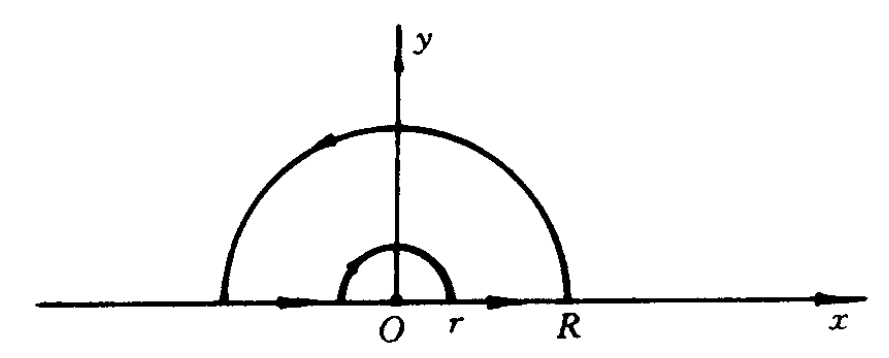
\includegraphics[width=0.6\textwidth]{images/9.png}
  \caption{题\ref{9}的图示.}
  \label{fig:9}
\end{figure}

\begin{solution}
  令\(f(z)=\frac{e^{2iz}-1}{z^2}\). 考虑图\ref{fig:9}中围道. 则\[\int_{-R}^{-r}-\int_{\gamma_r}+\int_{r}^R+\int_{\gamma_R} f(z)dz=:I_1-I_2+I_3+I_4=0.\]

  作换元\(x\to -x\), \[I_1+I_3=\int_r^R \frac{e^{-2ix}-1}{x^2}dx+\int_r^R \frac{e^{2ix}-1}{x^2}dx=-4\int_r^R \left(\frac{\sin x}{x}\right)^2dx.\]

  由Jordan引理, \[\lim_{R\to\infty} I_4=0.\]

  由引理5.5.9, \[\lim_{r\to0}I_2=i\pi\lim_{z\to0}zf(z)=-2\pi.\]

  令\(R\to\infty\), \(r\to0\)得\(-4I+2\pi=0\), 即\[I=\frac{\pi}{2}.\tag*{\(\qed\)}\]
  \renewcommand{\qedsymbol}{}
\end{solution}

\begin{problem}[5.5.1(11)] \label{11}
  计算\[I=\int_0^\infty \frac{x^p}{1+x^2}dx,\] 其中\(-1<p<1\).
\end{problem}

\begin{figure}[htbp]
  \centering
  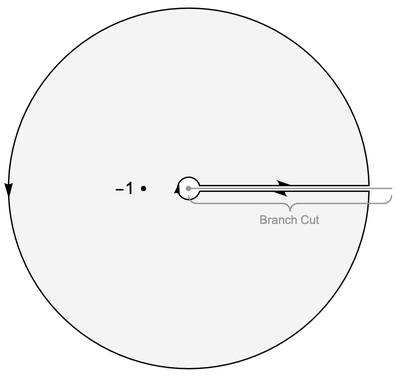
\includegraphics[width=0.4\textwidth]{images/11.png}
  \caption{题\ref{11}的图示.}
  \label{fig:11}
\end{figure}

\begin{solution}
  一般地, 对\(-1<a<b-1\), \(b>0\), 有\[I=\int_0^\infty \frac{x^a}{1+x^b}dx=\frac{\pi}{b}\csc\left(\pi\frac{a+1}{b}\right).\]

  作换元\(y=x^b\), \[I=\frac{1}{b}\int_0^\infty\frac{y^{(a+1-b)/b}}{1+y}dy.\]

  令\(f(z)=\frac{z^{(a+1-b)/b}}{1+z}\), 在正实轴上岸取正值. 考虑图\ref{fig:11}中围道. 则\[\int_{r}^{R}+\int_{\gamma_R}-\int_{\gamma_1}-\int_{\gamma_r} f(z)dz=:I_1+I_2-I_3-I_4=2\pi i\text{Res}(f,-1)=2\pi i e^{i\pi \frac{a+1-b}{b}}.\]

  当\(R\to\infty\)时, \[I_2=O\left(R^{\frac{a+1-b}{b}-1+1}\right)\to0.\]

  当\(r\to0\)时, \[I_4=O\left(r^{\frac{a+1-b}{b}}r\right)\to0.\]

  对\(x\in(0,\infty)\), \[f(x_{\text{下}})=f(x_{\text{上}})\exp\left(2i\pi\frac{a+1-b}{b}\right),\] 从而\[I_3=I_1\exp\left(i\pi\frac{a+1-b}{b}\right).\]

  令\(R\to\infty\), \(r\to 0\), 得\[b\left(1-e^{2i\pi \frac{a+1-b}{b}}\right)I=2\pi i e^{i\pi \frac{a+1-b}{b}}.\]

  取虚部可得\[I=\frac{\pi}{b}\csc\left(\pi\frac{a+1}{b}\right). \tag*{\(\qed\)}\]
  \renewcommand{\qedsymbol}{}
\end{solution}

\begin{problem}[5.5.1(15)]\label{15}
  计算\[I=\int_0^1 \frac{x^{1-p}(1-x)^p}{1+x^2}dx,\] 其中\(-1<p<2\).
\end{problem}

\begin{figure}[htbp]
  \centering
  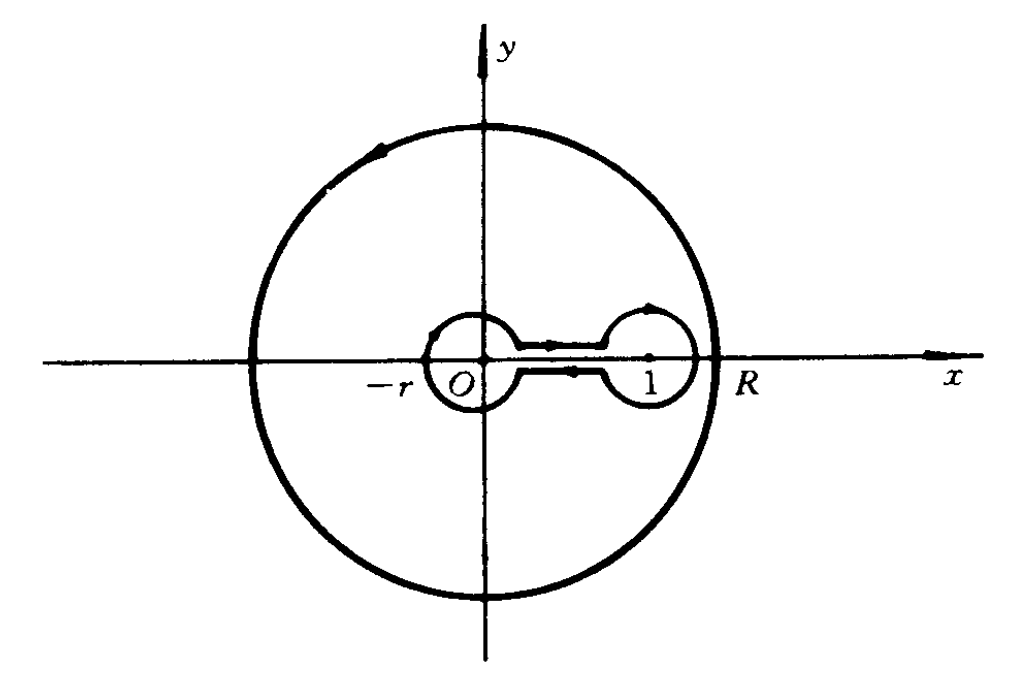
\includegraphics[width=0.6\textwidth]{images/15.png}
  \caption{题\ref{15}的图示.}
  \label{fig:15}
\end{figure}

\begin{solution}
  令\(f(z)=\frac{z^{1-p}(1-z)^p}{1+z^2}\), 在\((0,1)\)上岸取正实数. 考虑图\ref{fig:15}中围道. 则\[\int_{r}^{1-r}+\int_{\gamma_2}-\int_{\gamma_3}-\int_{\gamma_r}+\int_{\gamma_R} f(z)dz=:I_1+I_2-I_3-I_4+I_5=2\pi i\left(\text{Res}(f,i)+\text{Res}(f,-i)\right)\]

  计算留数: \[\text{Res}(f,i)=\lim_{z\to i}\frac{z^{1-p}(1-z)^p}{z+i}=\frac{1}{2i}2^{p/2}\exp i\left((1-p)\cdot\frac{\pi}{2}+p\cdot(-\frac{\pi}{4})\right)=2^{\frac{p}{2}-1}e^{-\frac{3p\pi i}{4}},\] \[\text{Res}(f,-i)=\lim_{z\to -i}\frac{z^{1-p}(1-z)^p}{z-i}=-\frac{1}{2i}2^{p/2}\exp i\left((1-p)\cdot\frac{3\pi}{2}+p\cdot\frac{\pi}{4}\right)=2^{\frac{p}{2}-1}e^{-\frac{5p\pi i}{4}}.\]

  当\(R\to\infty\)时, 由引理5.5.15, \[I_5\to2\pi i e^{-i\pi p}.\]

  当\(r\to0\)时, \[I_4=O(r^{1-p}r)\to 0,\] \[I_2=O(r^p r)\to0.\]

  对\(x\in(0,1)\), \[f(x_{\text{下}})=f(x_{\text{上}})e^{-2i\pi p},\] 从而\[I_3=I_1e^{-2i \pi p}.\]

  令\(R\to\infty\), \(r\to 0\), \[(1-e^{-2i\pi p})I+2\pi ie^{-i\pi p}=i\pi 2^{\frac{p}{2}}\left(e^{-i\frac{3\pi p}{4}}+e^{-i\frac{5\pi p}{4}}\right).\]

  取虚部可得\[I=-\frac{\pi}{\sin p\pi}+\frac{\pi 2^{p/2}\cos \frac{p\pi}{4}}{\sin p\pi}. \tag*{\(\qed\)}\]
  \renewcommand{\qedsymbol}{}
\end{solution}

\begin{problem}[5.5.1(21)]\label{21}
  计算\[I=\int_0^\infty \frac{\log x}{x^2-1}dx.\]
\end{problem}

\begin{figure}[htbp]
  \centering
  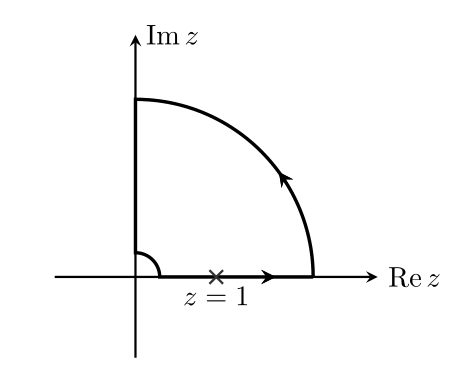
\includegraphics[width=0.4\textwidth]{images/21.png}
  \caption{题\ref{21}的图示.}
  \label{fig:21}
\end{figure}

\begin{solution}
  令\(f(z)=\frac{\log z}{z^2-1}\). 考虑图\ref{fig:21}中围道. 则\[\int_{r}^{R}+\int_{\gamma_R}-\int_{ri}^{Ri}-\int_{\gamma_r} f(z)dz=:I_1+I_2-I_3-I_4=0.\]

  令\(z=yi\), \[I_3=\int_r^R\frac{\log y+\frac{\pi}{2}i}{-y^2-1}idy=\frac{\pi}{2}\int_r^R\frac{dy}{1+y^2}+\text{虚数}.\]

  当\(R\to\infty\)时, \[I_2=O\left(\frac{\log R}{R^2}\cdot R\right)\to0.\]

  当\(r\to0\)时, \[I_4=O\left(\frac{\log r}{1-r^2}\cdot r\right)\to0.\]

  令\(R\to\infty\), \(r\to0\)并取实部得\[I=\frac{\pi}{2}\int_0^\infty\frac{dy}{1+y^2}=\frac{\pi^2}{4}.\tag*{\(\qed\)}\]
  \renewcommand{\qedsymbol}{}
\end{solution}

\begin{problem}[5.5.1(25)] \label{25}
  计算\[I=\int_0^\infty \frac{x}{e^x+1}dx.\]
\end{problem}

\begin{figure}[htbp]
  \centering
  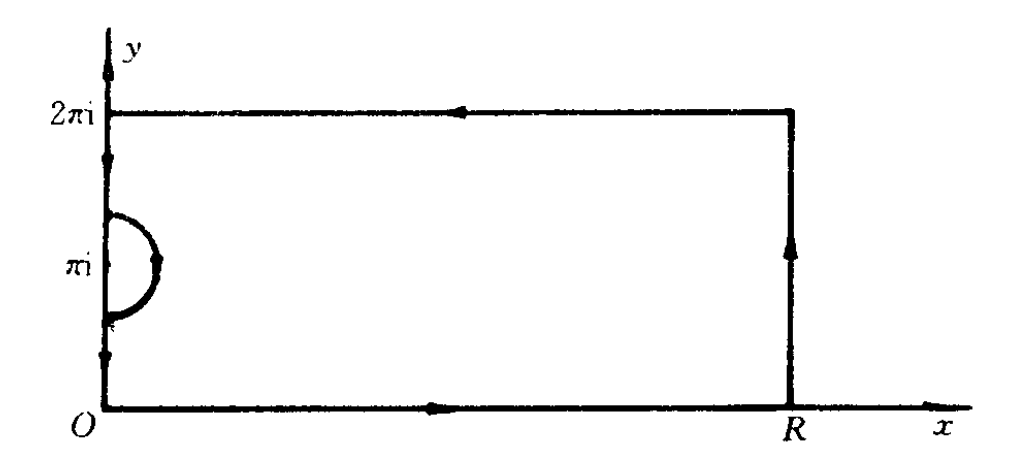
\includegraphics[width=0.6\textwidth]{images/25.png}
  \caption{题\ref{25}的图示.}
  \label{fig:25}
\end{figure}

\begin{solution}
  令\(f(z)=\frac{z^2}{e^z+1}\). 考虑图\ref{fig:25}中围道. 则\[\int_{0}^{R}+\int_{\gamma_1}+\int_{R+2\pi i}^{2\pi i}-\int_{\pi i}^{2\pi i}-\int_{\gamma_2}-\int_{0}^{\pi i} f(z)dz=:I_1+I_2+I_3-I_4-I_5-I_6=0.\]

  令\(z=x+2\pi i\), \[I_1+I_3=\int_0^R\left(\frac{x^2}{e^x+1}-\frac{(x+2\pi i)^2}{e^x+1}\right)dx=-4\pi^2\int_0^R\frac{1}{e^x+1}dx-4\pi i\int_0^R \frac{x}{e^x+1}dx.\]

  当\(R\to\infty\)时, \[I_2\to 0.\]

  令\(z=ix\), \begin{align*}I_4+I_6&=\int_{0}^{\pi-r}+\int_{\pi+r}^{2\pi} \frac{(xi)^2}{e^{xi}+1}idx=-\int_{0}^{\pi-r}+\int_{\pi+r}^{2\pi}\frac{ix^2(1+\cos x-i\sin x)}{2+2\cos x}dx\\&=\text{实数}-i\left(\frac{4\pi^3}{3}+\frac{1}{6}(\pi-r)^3-\frac{1}{6}(\pi+r)^3\right).\end{align*}

  由引理5.5.9, \[\lim_{r\to\infty}I_5=i\pi\lim_{z\to\pi i}f(z-\pi i)f(z)=\pi^3.\]

  令\(R\to\infty\), \(r\to0\)并取虚部得\[-4\pi I+\frac{4\pi^3}{3}-\pi^3=0,\]
  即\[I=\frac{\pi^2}{12}. \tag*{\(\qed\)}\]
  \renewcommand{\qedsymbol}{}
\end{solution}

\section{补充题}

\begin{problem}[5.2.6]
  设\(f\)是\(B(z_0,R)\backslash\{z_0\}\)上非常值的全纯函数. 证明: 若\(z_0\)是\(f\)的零点集的极限点, 则\(z_0\)是\(f\)的本性奇点.
\end{problem}

\begin{proof}
  由条件易知\(z_0\)是\(f\)的孤立奇点.
  
  若\(z_0\)是\(f\)的可去奇点, 则由\(z_0\)是\(f\)的零点集的极限点知\(\lim_{z\to _0}f(z)=0\), 且补充定义\(f(z_0)=0\)后\(f\)在\(B(z_0,R)\)全纯. 由唯一性定理知\(f\equiv0\), 矛盾.
  
  若\(z_0\)是\(f\)的极点, 则对\(B(z_0,R)\backslash\{z_0\}\)任意趋于\(z_0\)的序列\(\{w_n\}\), 有\(\lim_{n\to\infty}f(w_n=\infty)\), 与\(z_0\)是\(f\)的零点集的极限点矛盾.
  
  故\(z_0\)是\(f\)的本性奇点.
\end{proof}

\begin{problem}[5.2.7]
  若\(f\)是\(B(z_0,R)\backslash\{z_0\}\)上的亚纯函数, 且\(z_0\)是\(f\)的极点集的极限点, 则对任意\(A\in\mathbb{C}_\infty\), 存在\(B(z_0,R)\backslash\{z_0\}\)中收敛于\(z_0\)的点列\(\{z_n\}\), 使得\(\lim_{n\to\infty}f(z_n)=A\).
\end{problem}

\begin{proof}
  设题中所说点列为\(\{w_n\}\).

  若\(A=\infty\), 则对任意\(n\), 由于\(w_n\)是极点, 存在\(z_n\in B(z_0,R)\backslash\{z_0\}\), 使得\(|z_n-w_n|<\frac1n\)且\(|f(z_n)>n\). 从而\(z_n\to z_0\)且\(\lim_{n\to\infty}f(z_n)=\infty=A\).

  设\(A\)是有限. 若\(z_0\)任一邻域中有\(f(z)-A\)的零点, 则结论成立. 若不然, 存在\(\delta>0\), 使得\(f(z)-A\)在\(0<|z-z_0|<\delta\)中恒不为\(0\). 令\(g(z)=\frac{1}{f(z)-A}\), \(0<|z-z_0|<\delta\). 对\(f\)的任一极点\(w\), \(\lim_{z\to w}g(z)=0\), 补充定义\(g(w)=0\), 则\(g\)在\(B(z_0,\delta)\backslash\{z_0\}\)中全纯. 因为\(\lim_{n\to\infty}g(w_n)=0\), 所以\(z_0\)或者是\(g\)的本性奇点, 或者是可去奇点. 下面讨论这两种情况.

  若\(z_0\)是\(g\)的可去奇点, 则补充定义\(g(z_0)=0\), \(g\)在\(B(z_0,\delta)\)中全纯. 由唯一性定理, \(g\equiv0\), 与\(f\)在\(B(z_0,R)\backslash\{z_0\}\)上亚纯矛盾.

  若\(z_0\)是\(g\)的本性奇点, 则存在\(B(z_0,R)\backslash\{z_0\}\)中收敛于\(z_0\)的点列\(\{z_n\}\), 使得\(g(z_n)\to\infty\), 从而\(f(z_n)\to A\), 结论成立.
\end{proof}

\begin{problem}[5.2.8]
  设\(f\)在\(B(0,R)\backslash\{0\}\)上全纯. 证明: 若\(\Re f(z)>0\)对所有\(z\in B(0,R)\backslash\{0\}\)成立, 则\(0\)是\(f\)的可去奇点.
\end{problem}

\begin{proof}
  由条件易知\(0\)是\(f\)的孤立奇点. 令\(g(z)=\frac{f(z)-1}{f(z)+1}\), 则\(g\)在\(B(0,R)\backslash\{0\}\)上全纯, \(0\)是\(g\)的孤立奇点.

  由\(\Re f(z)>0\)可得\(|g(z)|<1\), 从而\(0\)是\(g\)的可去奇点. 因此\(\lim_{z\to0}g(z)=A\in\mathbb{C}\backslash\{1\}\). 

  故\(\lim_{z\to0}f(z)=\frac{1+A}{1-A}\), 从而\(0\)是\(f\)的可去奇点.
\end{proof}

\begin{problem}[5.3.5]
  设\(f\)是整函数, 证明:
  \begin{enumerate}
    \item 若\(f(\mathbb R)\subset \mathbb{R}\), \(f(i\mathbb R)\subset i\mathbb R\), 则\(f\)是奇函数;
    \item 若\(f(\mathbb R)\subset \mathbb R\), \(f(i\mathbb R)\subset \mathbb R\), 则\(f\)是偶函数.
  \end{enumerate}
\end{problem}

\begin{proof}
  \begin{enumerate}
    \item 令\(g(z)=f(z)-\overline{f(\overline z)}\), \(g\)是整函数. 任意\(x\in\mathbb R\), \(f(x)=\overline{f(x)}=\overline{f(\overline x)}\), 即\(g(x)=0\). 从而\(g\equiv 0\), 即\(f(z)\equiv\overline{f(\overline{ z})}\).
    
    令\(h(z)=f(z)+f(-z)\). 任意\(x\in\mathbb R\), \(f(-xi)=\overline{f(xi)}=-f(xi)\), 即\(h(x)=0\). 从而\(h\equiv0\). 
    
    故\(f\)是奇函数.

    \item 同1可知\(f(z)\equiv\overline{f(\overline{ z})}\).
    
    令\(h(z)=f(z)-f(-z)\). 任意\(x\in\mathbb R\), \(f(-xi)=\overline{f(-xi)}=f(xi)\), 即\(h(x)=0\). 从而\(h\equiv0\). 
    
    故\(f\)是偶函数.\qed
  \end{enumerate}
  \renewcommand{\qedsymbol}{}
\end{proof}

\begin{problem}[5.4.3]
  设\(f\)在\(B(\infty,R)\)上全纯, 证明:
  \begin{enumerate}
    \item 若\(\infty\)是\(f\)的可去奇点, 则\[\text{Res}(f,\infty)=\lim_{z\to\infty}z^2f'(z);\]
    \item 若\(\infty\)是\(f\)的\(m\)阶极点, 则\[\text{Res}(f,\infty)=\frac{(-1)^m}{(m+1)!}\lim_{z\to\infty}z^{m+2}f^{(m+1)}(z).\]
  \end{enumerate}
\end{problem}

\begin{proof}
  \begin{enumerate}
    \item 令\(g(z)=f(1/z)\). \(0\)是\(g\)的可去奇点. 于是\begin{align*}
      \text{Res}(f,\infty)&=-\frac{1}{2\pi i}\int_{|z|=R_0} f(z)dz\\
      &=-\frac{1}{2\pi i}\int_{|z|=\frac{1}{R_0}} \frac{g(z)}{z^2}dz\\
      &=-g'(0)\\
      &=-\lim_{z\to0}g'(z)\\
      &=\lim_{z\to 0}\frac{f'(1/z)}{z^2}\\
      &=\lim_{z\to\infty}z^2f'(z).
    \end{align*}
    \item 可设\(f\)的Laurent展开为\[f(z)=a_mz^m+a_{m-1}z^{m-1}+\cdots.\]
    因此\[\text{Res}(f,\infty)=-a_{-1}=\frac{(-1)^m}{(m+1)!}\lim_{z\to\infty}z^{m+2}f^{(m+1)}(z).\tag*{\(\qed\)}\]
  \end{enumerate}
  \renewcommand{\qedsymbol}{}
\end{proof}

\section{概率分布特征函数的计算}

\begin{problem}[正态分布]
  设\(X\sim N(\mu,\sigma^2)\), 有p.d.f. \[f(x)=\frac{1}{\sqrt{2\pi}\sigma}e^{-\frac{(x-\mu)^2}{2\sigma^2}}.\] 则其特征函数为\[\phi(t)=\exp\left(i\mu t-\frac12 \sigma^2t^2\right).\]
\end{problem}

\begin{proof}
  令\(y=\frac{x-\mu}{\sigma}\), 则\[
    \phi(t)=\int_{-\infty}^\infty e^{itx}f(x)dx=e^{i\mu t-\frac12\sigma^2t^2}\frac{1}{\sqrt{2\pi}}\int_{-\infty}^\infty e^{-\frac{(y-it\sigma)^2}{2}}dy.\]

  只需证明\[\int_{-\infty}^\infty e^{-\frac{(y-it\sigma)^2}{2}}dy=\sqrt{2\pi}.\]

  令\(f(z)=e^{-\frac{(z-it\sigma)^2}{2}}\). 考虑以\(\Im z=0\)和\(\Im z=t\sigma\)为上下边, 宽为\(2R\)的关于虚轴对称的矩形围道. 由Cauchy积分定理, \(f\)沿围道积分为\(0\). 而在两竖边上, \(|f(z)|=O(e^{-R^2})\). 令\(R\to\infty\), 有\[\int_{-\infty}^\infty e^{-\frac{(y-it\sigma)^2}{2}}dy=\int_{-\infty}^\infty e^{-\frac{y^2}{2}}dy=\sqrt{2\pi}.\tag*{\(\qed\)}\]
  \renewcommand{\qedsymbol}{}
\end{proof}

\begin{problem}[Gamma分布]
  设\(X\sim \text{Gamma}(\alpha,\beta)\), 有p.d.f. \[f(x)=\frac{\beta^\alpha}{\Gamma(\alpha)}x^{\alpha-1}e^{-\beta x},\] 其中\(\alpha>0\), \(\beta>0\), \(\Gamma(\alpha)=\int_0^\infty t^{\alpha-1}e^{-t}dt\). 则其特征函数为\[\phi(t)=\left(1-\frac{it}{\beta}\right)^{-\alpha}.\] 
\end{problem}

\begin{proof}
  令\(f(z)=z^{\alpha-1}e^{(it-\beta)z}=e^{(\alpha-1)\log z+(it-\beta)z}\). 则\[\phi(x)=\frac{\beta^\alpha}{\Gamma(\alpha)}\int_0^\infty f(x)dx.\]

  考虑扇形围道, 半径为\(R\), 两边为正实轴和\(\{z=\frac{x}{-it+\beta}:x\ge0\}\), 且在原点附近去掉半径为\(r\)的小圆弧. 由Cauchy积分定理, \(f\)沿围道积分为\(0\).

  沿大圆弧, \(|f(z)|\)关于\(R\)指数衰减, 从而积分趋于\(0\).
  
  沿小圆弧, \(|f(z)|=O(r^{\alpha-1})\), 从而积分趋于\(0\).

  令\(R\to\infty\), \(r\to0\), 有\[\int_0^\infty f(x)dx=\int_0^\infty f\left(\frac{x}{-it+\beta}\right)\frac{1}{-it+\beta}dx=\Gamma(\alpha)\left(\frac{1}{\beta-it}\right)^\alpha.\]

  故\[\phi(t)=\left(1-\frac{it}{\beta}\right)^{-\alpha}.\tag*{\(\qed\)}\]
  \renewcommand{\qedsymbol}{}
\end{proof}

\end{document}